\documentclass[10pt]{article}

\usepackage{lipsum}
\usepackage{url}
\usepackage{float}
\usepackage{amsmath}
\usepackage{enumitem}
\usepackage{graphicx}
\usepackage{caption}
\usepackage{subcaption}
\usepackage{rotating}
\usepackage{geometry}
\usepackage{listings}
\usepackage{hyperref}
\usepackage[T1]{fontenc}
\usepackage[numbered]{matlab-prettifier}

\newcommand{\documentTitle}{Lab 6 - Digital Signal Processing}
\newcommand{\documentAuthor}{Andrew Pham, Aneel Damaraju}
\newcommand{\courseTitle}{ELEC 240}
\newcommand{\testDate}{October 16, 2018}
\newcommand{\reportDate}{October 23, 2018}

\geometry{margin=1in}
\lstset{
    tabsize=4,
    basicstyle={\ttfamily},
    captionpos=b,
    belowskip=1em,
    aboveskip=1em,
    numbers=left,
	escapechar=\@,
}

\title{
    \textbf{\courseTitle} \\
    \textbf{\documentTitle} \\
    \bigskip
    \textbf{\large{Test performed: \testDate}} \\
    \textbf{\large{Report submitted: \reportDate}} \\
    \bigskip
    \bigskip
}
\author{\documentAuthor}
\date{}

\begin{document}

\maketitle

\newpage

\section{Objective}

The first objective of this lab was to understand the key concepts behind sampling, through use of varying the sampling frequency and input frequency of a given signal. There was also some inspection into another important factor in digital signal processing, quantization, and seeing how effective a quantized signal recreates an input. The second objective was more skills based, focusing on learning how to upload vocal signals to MATLAB through LabView. This included understanding the specgram and sound functions in MATLAB, as well qualitatively understanding some key features of spectral plots. For the final objective, we focused on learning about various types of filters and their frequency and unit sample responses.

\medskip
\section{Materials}
\begin{itemize}
	\item Virtual Bench (Software, Oscilloscope, Function Generator, DC Power Supply)
	\item LabView
	\item BNC Male to Clips cord
	\item Oscilloscope Probe
	\item Breadboard (with setup from Lab 4
	\item 2 10 cm length wires (with 6 mm stripped on each end)
	\item Digital Multimeter
	\item 100 $k\Omega$ resistor
	\item 2 100 $\Omega$ resistors
	\item 1 $k\Omega$ resistor
	\item 2 LM 741 Op-Amps
	\item Telephone handset
	\item Dynamic microphone
	\item Smartphone (or some device to play audio from a speaker)
	\item MATLAB
	\item Lab PC
\end{itemize}


\section{Test Description}

In Experiment 6.1, Part A, we connected the function generator to a LabView spectrum analyzer, and varied the input function. We created a sine wave and varied the frequency of it as well as the sampling frequency and checked what properties of the sampled wave would change. We focused on the fundamental frequency and how the output looked around the Nyquist frequency. For Part B, we added a quantizer to our spectrum analyzer and compared the quantized signal to the original signal. From there, we changed the number of quantized bits and qualitatively viewed the output.

In Experiment 6.2, Part A, we created two Op-Amp circuits, one connecting the Lab PC sound card to the handset and one connecting the dynamic microphone to the DAQ cable. We then recorded two sounds, one being general human voice and the other being a single pitch whistle. For Part B, we simply loaded the signals into MATLAB and made sure that MATLAB could effectively recreate the now quantized sounds. For Part C, we took the signals and then plotted the magnitude of the signal as well as just a chunk of the signal.

In Experiment 6.3, Part A, we made changes to the signals amplitude and frequency and listened to the changes. We then added the two signals. For Part B, applied simple filters to the voice output, including cariable length boxcar filters and infinite impulse response filters. We found the unit sample, frequency and sound responses for each filter. For Part C, the same tests were done, but for the more complicated Butterworth and Finite Impulse responses.
 

\subsection{Pre-Lab Calculations and Schematics}

The Pre-Lab for this lab only included a general understanding of LabView and Virtual Bench, which was done in previous labs. The other information in this lab, is expected to be learned through examples found in the lab. 

\section{Results and Discussion}

In Experiment 6.1, Part A, we explored sampling a signal in the time domain. We began by connecting the function generator to pin 46, which was the input to the LabView software and generated a 5 $V_{pp}$, 300 Hz sine wave. We then sampled the signal at a rate of 10000 samples per second with average set to RMS averaging to achieve the following waveform graph in Fig \ref{fig:firstsample} below. 

\begin{centering}
	\begin{figure} [H]
		\centering
		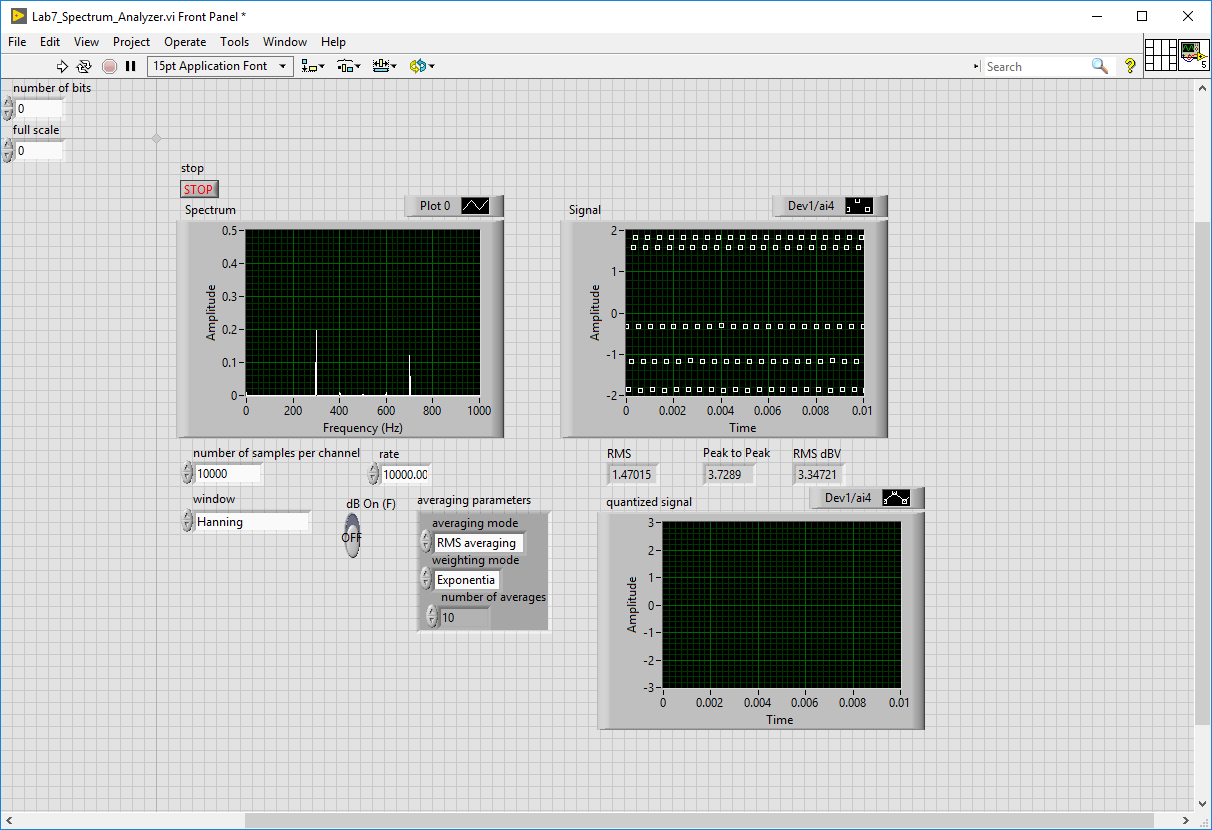
\includegraphics[scale=0.22]{images/61a2khzsample.PNG}
		\caption{Sample of 5 $V_{pp}$, 300 Hz Sine Wave}
		\label{fig:firstsample}
	\end{figure}
\end{centering}

We then began to increase the frequency of the sine wave outputted by the function generator. When the output frequency was half of the sampling frequency, we observed that the samples alternated between positive and negative values. We began to observe aliasing past 5kHz, and the input frequency stopped matching the displayed frequency in Labview. For example, in Fig \ref{fig:11khz} and Fig \ref{fig:13khz} below, we can observe aliasing when the input frequency is 11 kHz and 13 kHz, respectively. 

\begin{centering}
	\begin{figure} [H]
		\centering
		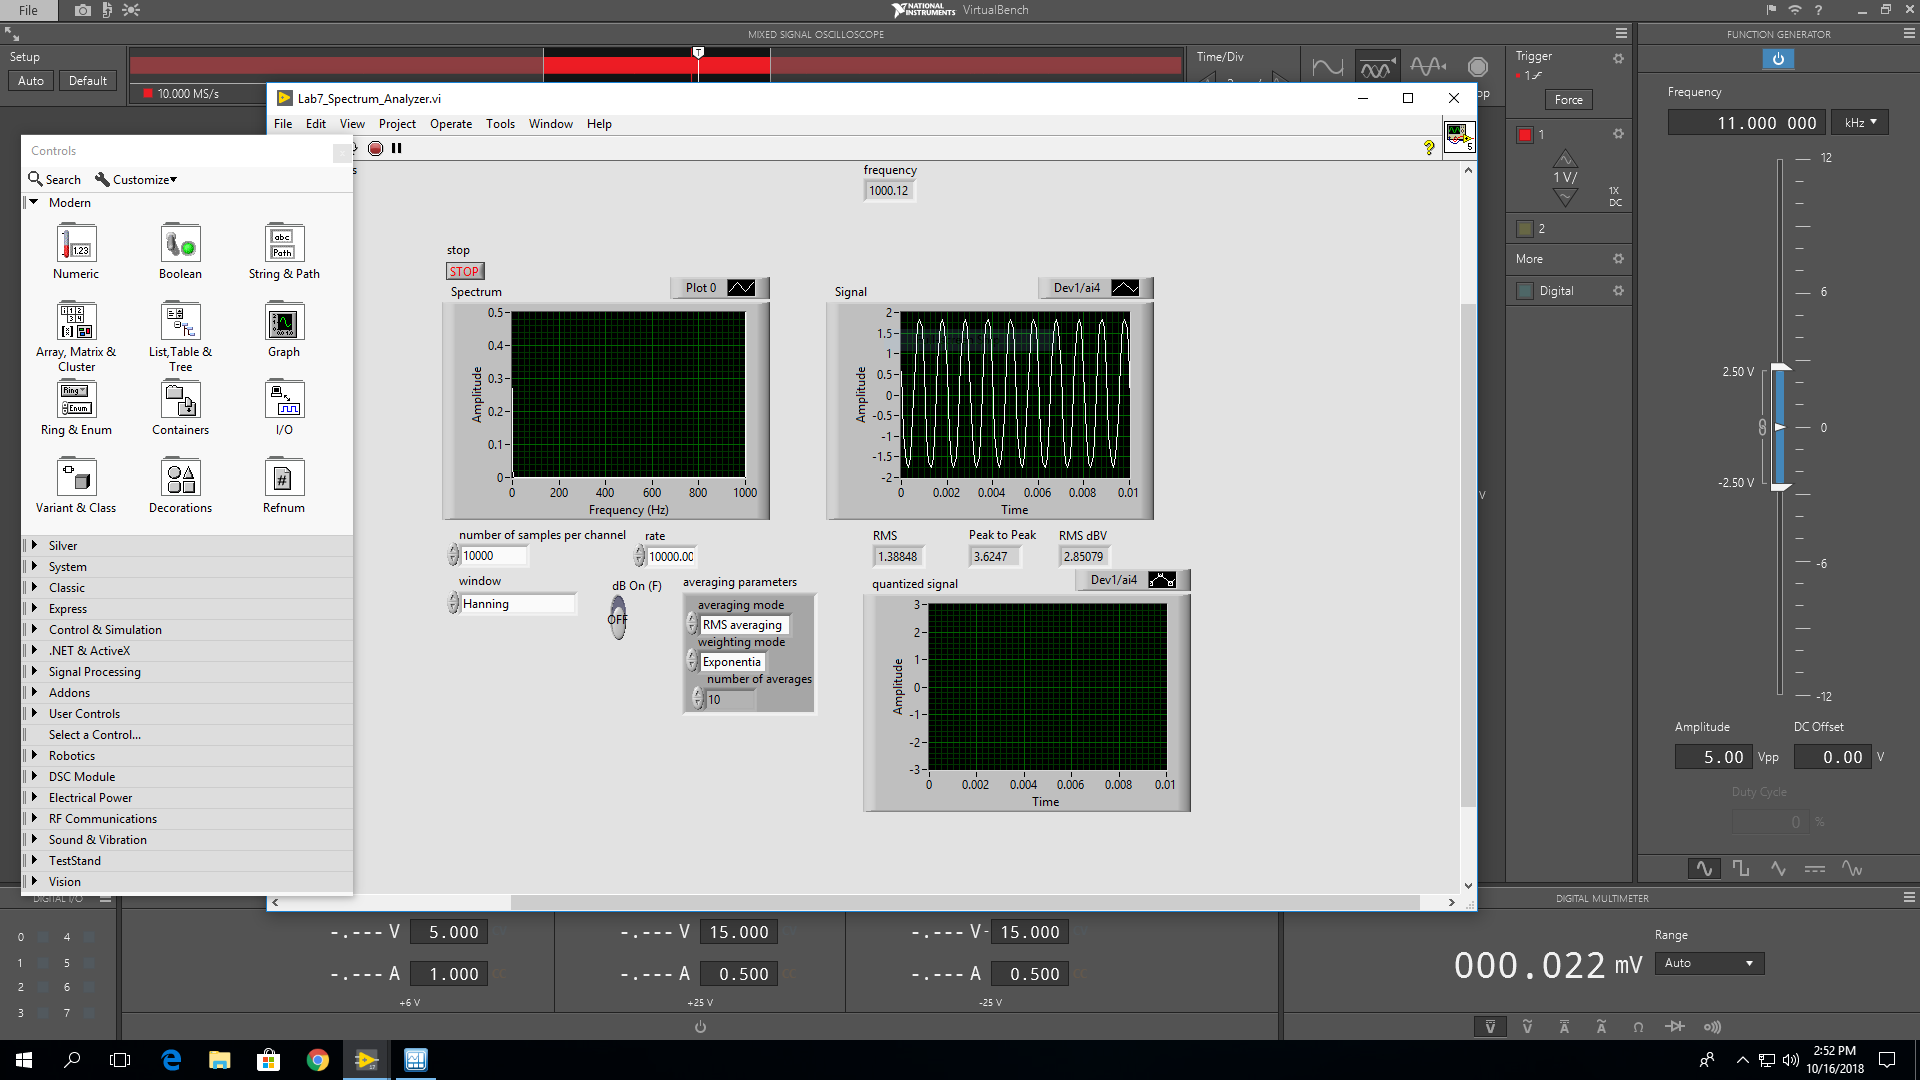
\includegraphics[scale=0.22]{images/51a11000input1000measured.PNG}
		\caption{10 kHz Sample of 11kHz Sine Wave}
		\label{fig:11khz}
	\end{figure}
\end{centering}

\begin{centering}
	\begin{figure} [H]
		\centering
		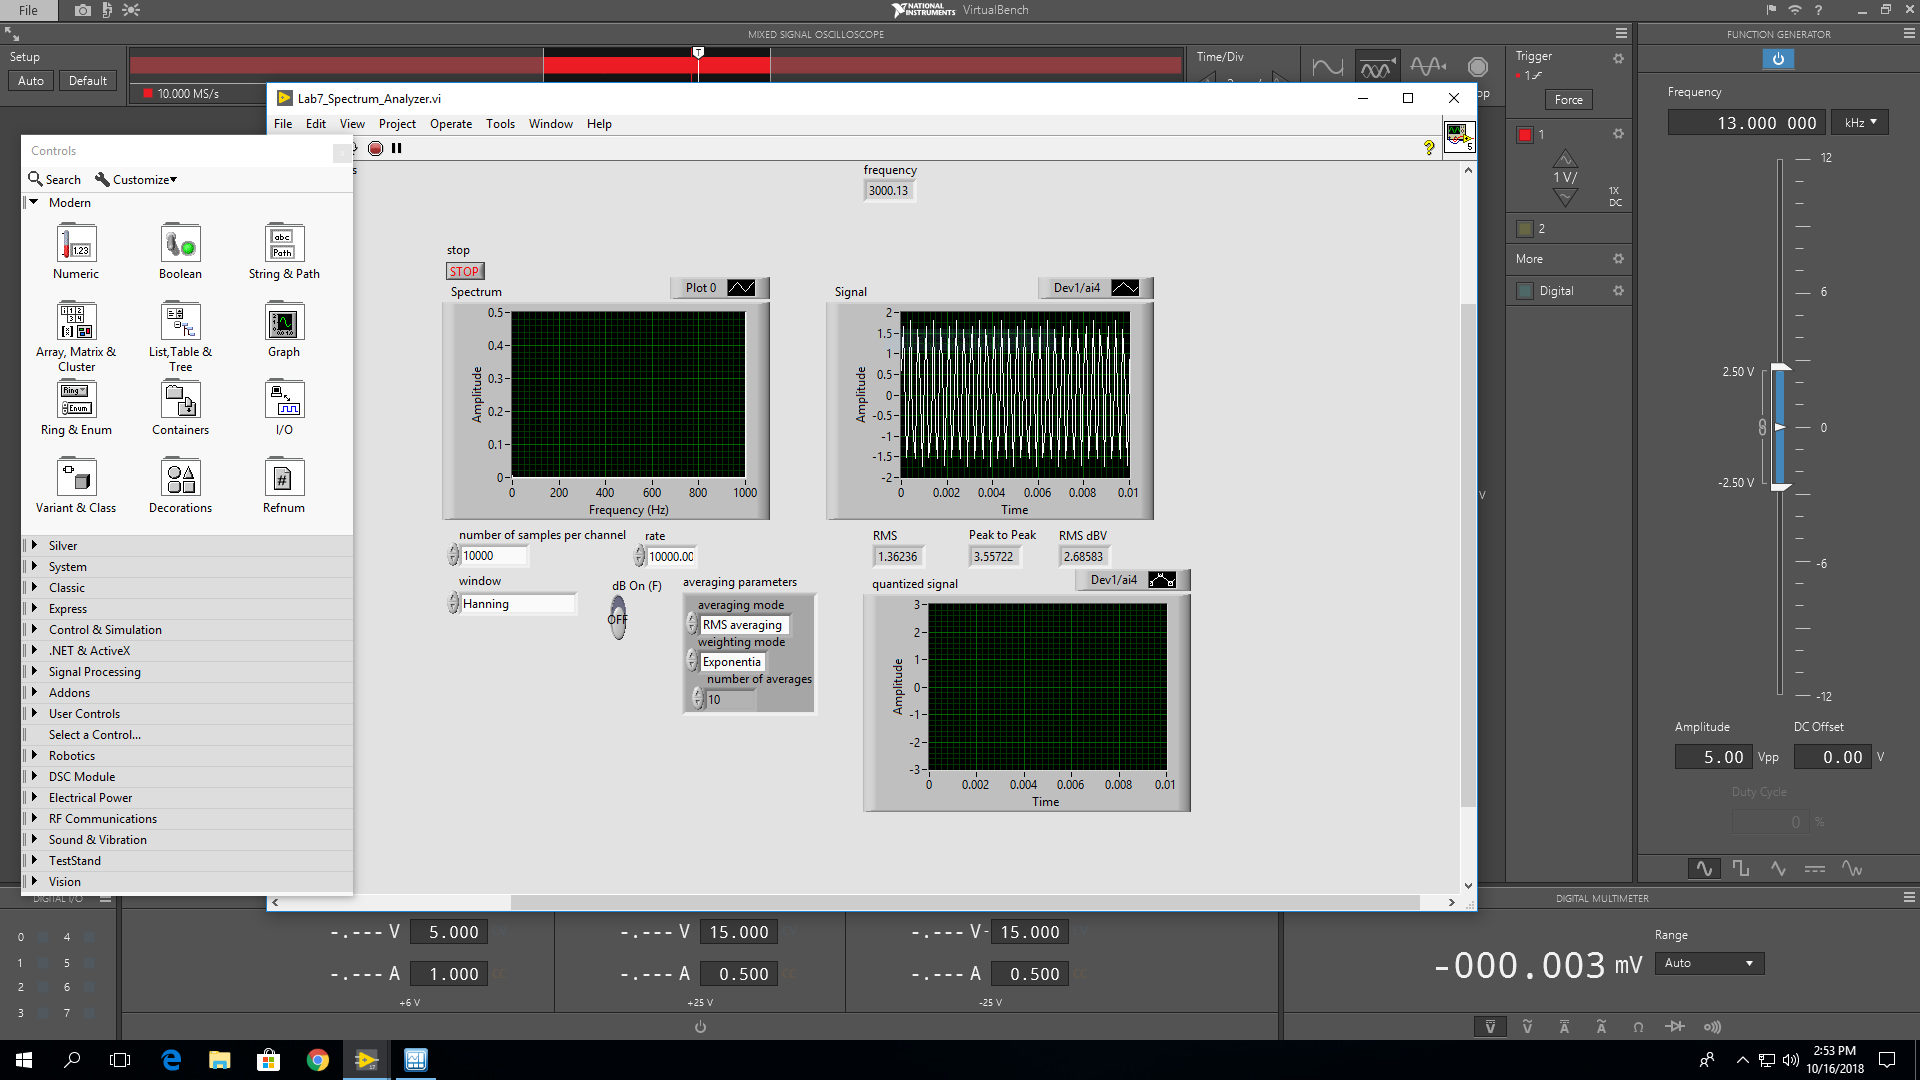
\includegraphics[scale=0.22]{images/51a13000input3000measured.PNG}
		\caption{10 kHz Sample of 11kHz Sine Wave}
		\label{fig:13khz}
	\end{figure}
\end{centering}

In the above figures, the output waveform is the alias of the input frequency, which occurs whenever twice the input frequency exceeds the sampling frequency. This concept is directly related to the Nyquist criterion, which states that no aliasing will occur as long as the sampling frequency is greater than or equal to twice the input frequency. Whenever the input frequency exceeds the Nyquist frequency, the input frequency is "folded over" into a lower. Thus, the 11 kHz signal was folded over the 10 kHz sampling frequency into a 1 kHz wave, and the 13 kHz signal was folded over the 10 kHz sampling frequency into a 3 kHz wave, as seen in the figures above. 

We then switched the function generator to produce a square wave and a sine wave. On frequencies that were integer divisors of the sampling frequency, the wave appeared to be sampled correctly below 5 kHz. However, on other frequencies such as 1.3 kHz, both the triangle and square wave appeared distorted. We attribute this distortion to the fact that neither square waves nor triangle waves are bandlimited, which means that the Nyquist Sampling theorem does not apply to them.


In Part B of Experiment 6.1, we explored amplitude quantization of discretely sampled signals. We began by producing a 1 kHz sine wave and feeding it into the amplitude quantizer that we constructed in Labview. As we increased the number of bits used by the quantizer, we noticed that the sampled sine wave became much more fluid and discerniblee. Likewise, as we decreased the number of bits, the sampled sine waveform became choppier and more step-like. We then switched the power spectrum graph to accept the discretely quantized sine wave as input rather than the original analog sine wave. We noticed that the amplitude of the power spectrum graph increased by 20\%. 


\medskip


\section{References}

\medskip

\section{Conclusion}

Your text here

\medskip

\textit{Note (To be deleted): While the ``Results and Discussion'' section focused on the test results individually, the ``Conclusion'' discusses the results in the context of the entire experiment. Usually, the objectives given in the ``Introduction'' are reviewed to determine whether the experiment succeeded. If the objectives were not met, you should analyze why the results were not as predicted.}

\section{Errors}
 
\end{document}
